\section{3D Pixel Development}
\subsection{Introduction}
This R\&D area covers sensors and electronics integrated utilizing 3-dimensional electronics technology.  This technology is distinct from 3D sensors and builds on efforts in the electronics industry to stack multiple layers of electronics to form dense assemblies of complex devices.  It is important for Particle Physics in that it allows very fine pitch (\unit[4]{\micron}) integration of sensors with multiple layers of electronics, allows interconnection to both the top and bottom of devices, and provides techniques for low mass, thinned devices. The interconnection of top and bottom means that sensors can be bonded to complex electronics with no wasted area for interconnect and optimal delivery of power and ground.
\subsection{Recent Milestones}
We have completed our multi-year effort to demonstrate commercial 3D technology. This consists of two tiers of \unit[0.13]{\micron} CMOS interconnected with Direct Oxide Bonding (DBI) technology and access using Through-Silicon-Vias (TSV). The DBI bonds are at \unit[4]{\micron} pitch. Fermilab sponsored the first 3D multi-project run for Particle Physics. The wafers were delivered last summer. Fermilab had three chips on the run: VICTR -- a CMS track trigger chip, VIPIC -- an X-ray imaging chip, and VIP -- an ILC vertex chip. Tests of the VIPIC and VICTR have shown working devices.  Tests for the VIP chip were delayed due to lack of funding and personnel.  We have recently restarted this work and initial tests are promising with the readout token successfully passed through the VIP.

In addition to the development of the 3D chips we have also explored the use of DBI to connect the 3D electronics with sensors.  Brookhaven Laboratory fabricated a sensor wafer with regions that mate to the VIP, VIPIC and VICTR chips.  The chips are ground to expose the top TSVs and contacts are deposited. The assembly is then attached to a handle wafer and the TSVs which project from the other side are exposed.  Wafers are then process for DBI bonding and individual die from the 3D wafer are bonded to the sensor wafer.  Finally the top ``handle'' silicon is ground and etched to reveal the previously formed contacts.  The total thickness of the readout at the end of this process is about \unit[25]{\micron} (Figure~\ref{fig:VertexDetector:VIP:chipsOnBNLWafer}). These wafers were received at the end of March 2014 and are being tested.
\begin{figure}
    \centering
    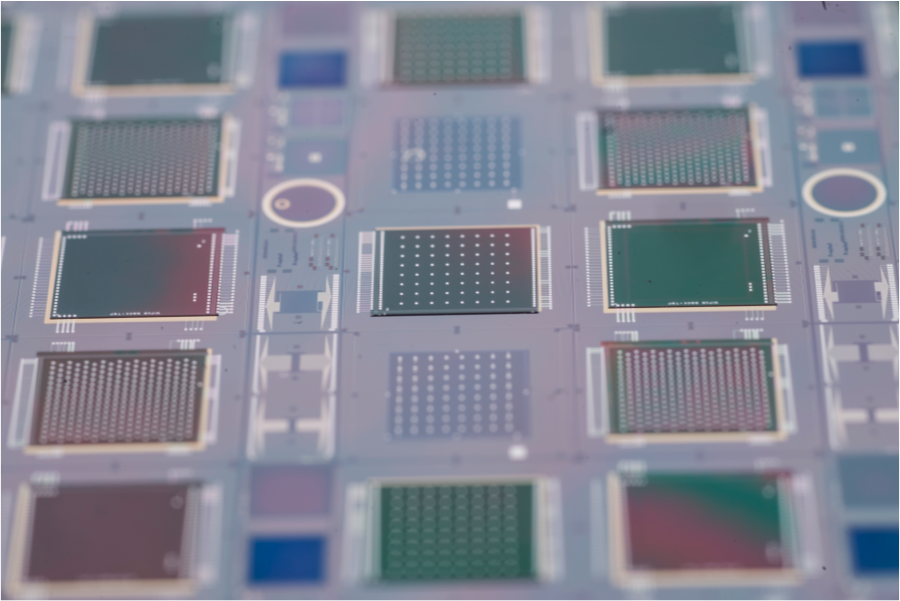
\includegraphics[width=0.5\textwidth]{VertexDetector/VIP/3DChipsOnBNLWafers}
\caption{3D chips placed on BNL sensor wafers. VIP is middle left and right}
\label{fig:VertexDetector:VIP:chipsOnBNLWafer}
\end{figure}
Due to the fact that contacts to a 3D assembly can be made to the body of the die, rather than its edge, no space needs to be reserved for wire bond contacts at the edge.  This raises the possibility of fabricating large, complex pixel detector arrays of 4-side butted devices using sensors with active edges.  We are in the process of demonstrating this technology utilizing active edge sensors fabricated at VTT and using wafer-to-wafer bonding to a 3D readout wafer. The active edge wafers are based on a silicon-on-insulator stack and thus can be fabricated with essentially arbitrarily thin sensors, in this case \unit[200]{\micron}. Sensor and dummy readout wafers have been fabricated and a test wafer is being etched at SLAC. We expect to have DBI bonded assemblies this summer.

\subsection{Engineering Challenges}
Major  engineering challenges include:
\begin{itemize}
\item Development of widely commercially available 3D technologies.  Based partly on our development the silicon brokers CMP, CMC, and MOSIS now include 3D multi-project runs as part of their standard offerings.
\item Development of high yield 3D bonded chip-to-wafer devices.  This is the subject of our active edge project.
\item This development shares with other vertexing technologies the problems of low mass mechanical support, power delivery, and cooling. An SOI-based device can be made thin without special effort. Such thinned device will need low mass backing hybrid circuitry, presumably flex on carbon fiber or a similar technology
\end{itemize}

\subsection{Future Plans}
\begin{itemize}
\item Complete the 3D active edge project
\item Apply our concepts to x-ray imaging devices
\item ILC developments would await renewed funding in the US.
\end{itemize}

\subsection{Applications outside of Linear Colliders}
As stated above the technology is already being developed for CMS and x-ray imaging applications.  The large area sensor concept is applicable for a variety of focal plane array concepts.

\begin{enumerate}
\item \fullcite{Deptuch:2013ona}
\item \fullcite{Yarema:2014mva}
\item \fullcite{MAJ:2013fwa}
\item \fullcite{2013arXiv1307.4301D}
\item \fullcite{1748-0221-7-12-C12010}
\item \fullcite{1748-0221-8-01-C01052}
\end{enumerate}
